% Chapter 02.9: নেটওয়ার্ক টপোলজি
\section{নেটওয়ার্ক টপোলজি}

\begin{learningbox}
এই টপিক শেষে শিক্ষার্থী পারবে:
\begin{itemize}
\item নেটওয়ার্ক টপোলজি কী তা ব্যাখ্যা করতে।
\item Physical topology ও Logical topology-এর ধারণা বুঝতে।
\item Bus, Star, Ring, Mesh, Tree ও Hybrid topology ব্যাখ্যা করতে।
\item বিভিন্ন topology-এর সুবিধা, অসুবিধা ও ব্যবহার লিখতে।
\item বাস্তব network scenario থেকে উপযুক্ত topology নির্বাচন করতে।
\item বোর্ড পরীক্ষার জন্য comparison-based answer, short answer ও CQ answer লিখতে।
\end{itemize}
\end{learningbox}

\subsection{বাস্তব জীবনের শুরু}

একটি computer lab কল্পনা করো। সেখানে ৩০টি computer, ১টি server, ১টি printer এবং internet connection আছে। এখন প্রশ্ন হলো—এই device-গুলো কীভাবে পরস্পরের সাথে যুক্ত হবে?

সব computer কি একটি central switch-এর সাথে যুক্ত হবে? নাকি একটি single cable-এর সাথে সবাই connect থাকবে? নাকি প্রতিটি device অন্য প্রতিটি device-এর সাথে আলাদা link দিয়ে যুক্ত থাকবে?

Network-এর device বা node-গুলো কীভাবে সাজানো ও সংযুক্ত থাকবে—এই arrangement-ই হলো \textbf{network topology}।

\begin{keypointbox}{মূল ধারণা}
Network topology বুঝতে তিনটি প্রশ্ন মনে রাখো:
\begin{itemize}
\item network-এর device বা node-গুলো কীভাবে connected?
\item data কোন path দিয়ে flow করছে?
\item কোনো link বা central device নষ্ট হলে network কতটা প্রভাবিত হবে?
\end{itemize}
\end{keypointbox}

\subsection{নেটওয়ার্ক টপোলজি}

\begin{definitionbox}{নেটওয়ার্ক টপোলজি}
কম্পিউটার নেটওয়ার্কে computer, server, switch, router, printer ইত্যাদি node বা device কীভাবে পরস্পরের সাথে যুক্ত ও বিন্যস্ত থাকে, সেই physical বা logical arrangement-কে network topology বলা হয়।
\end{definitionbox}

সহজভাবে, topology হলো network-এর layout বা structure। এটি network design, cost, performance, reliability, troubleshooting এবং scalability-এর উপর সরাসরি প্রভাব ফেলে।

\begin{examplebox}{সহজ উদাহরণ}
\begin{itemize}
\item Computer lab-এ সব PC যদি একটি switch-এর সাথে connected থাকে, তাহলে সেটি Star topology-এর উদাহরণ।
\item পুরনো network-এ সব computer একটি backbone cable-এর সাথে যুক্ত থাকলে সেটি Bus topology।
\item প্রতিটি node যদি অন্য প্রতিটি node-এর সাথে link দ্বারা connected থাকে, সেটি Mesh topology।
\end{itemize}
\end{examplebox}

\begin{figure}[H]
\centering
\IfFileExists{chapters/Chapter02/images/network_topology_basic_concept.png}{
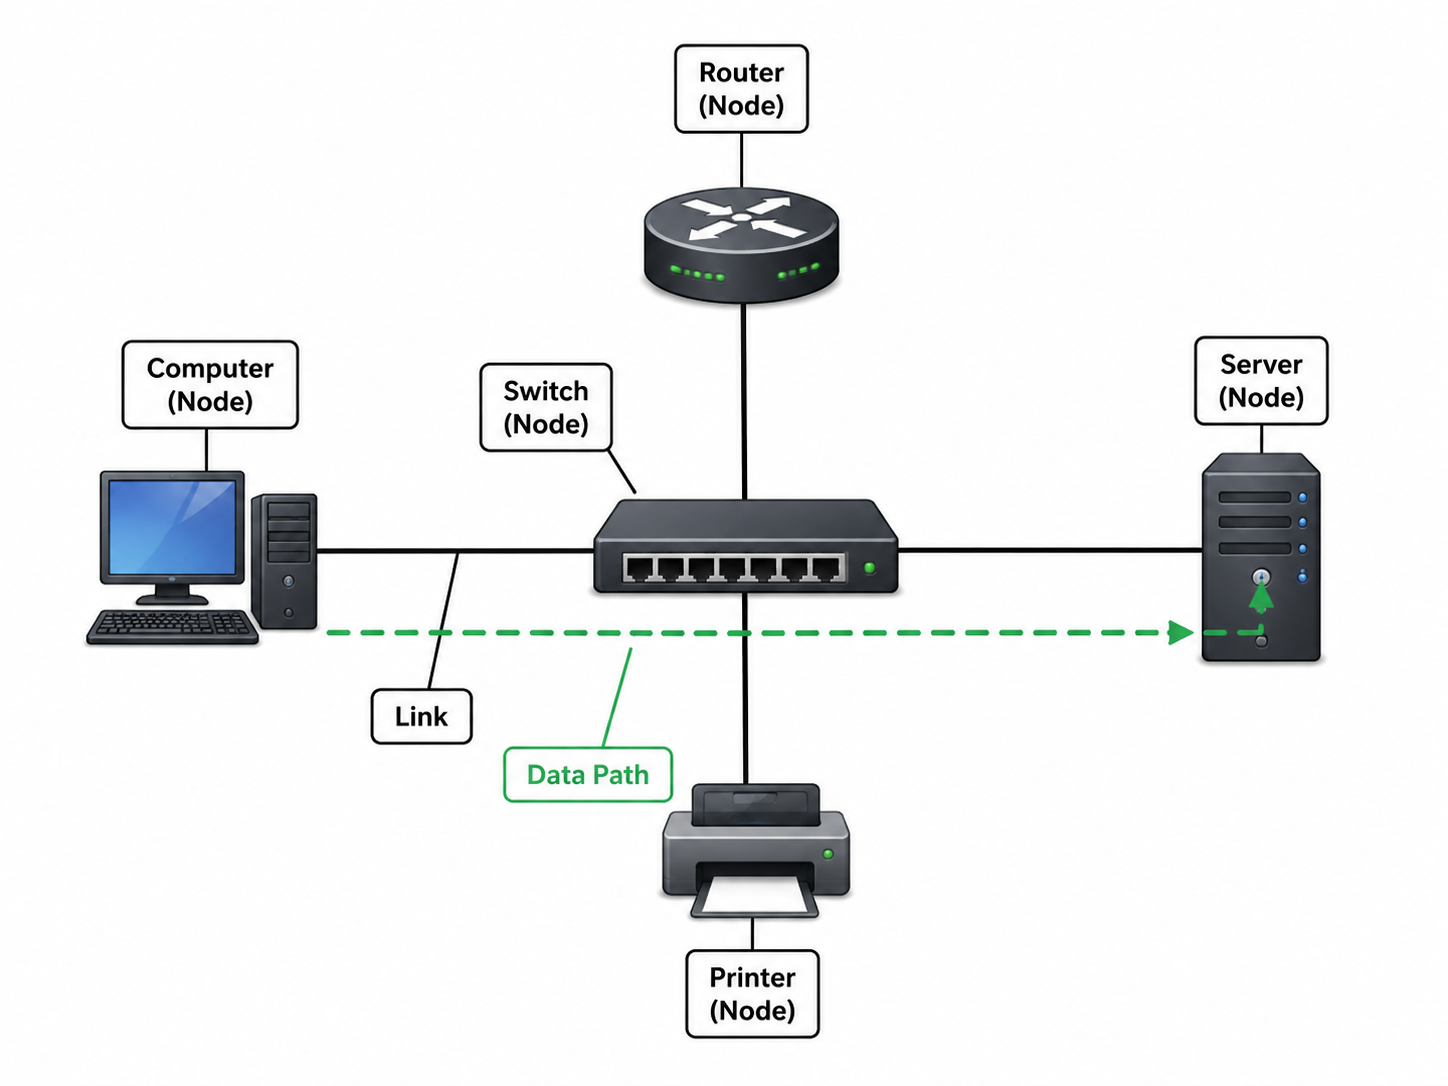
\includegraphics[width=0.92\textwidth]{chapters/Chapter02/images/network_topology_basic_concept.png}
}{
\fbox{
\parbox{0.90\textwidth}{
\centering
\vspace{0.7cm}
Network Topology[8pt]
Node + Link + Data Path[8pt]
Computer \quad Switch \quad Router \quad Server \quad Printer
\vspace{0.7cm}
}}
}
\caption{নেটওয়ার্ক টপোলজির মৌলিক ধারণা}
\end{figure}

\subsection{Network Topology কেন গুরুত্বপূর্ণ?}

একটি network কত দ্রুত কাজ করবে, কত সহজে manage করা যাবে, কোনো device নষ্ট হলে পুরো network বন্ধ হবে কি না, ভবিষ্যতে device add করা সহজ হবে কি না—এসব বিষয় topology-এর উপর নির্ভর করে।

\begin{keypointbox}{Topology গুরুত্বপূর্ণ কেন?}
\begin{itemize}
\item network design ও device placement বুঝতে সাহায্য করে।
\item network installation cost ও cable requirement নির্ধারণে সাহায্য করে।
\item data flow path বোঝা সহজ হয়।
\item fault finding বা troubleshooting সহজ হতে পারে।
\item network scalability বা ভবিষ্যতে expansion plan করা যায়।
\item failure হলে network কতটা প্রভাবিত হবে তা বিশ্লেষণ করা যায়।
\item performance ও traffic management-এর উপর প্রভাব ফেলে।
\end{itemize}
\end{keypointbox}

\subsection{Physical Topology ও Logical Topology}

Network topology দুইভাবে বোঝানো যায়:

\begin{itemize}
\item \textbf{Physical Topology}
\item \textbf{Logical Topology}
\end{itemize}

\begin{definitionbox}{Physical Topology}
Network-এর device, cable, switch, router ইত্যাদি hardware কীভাবে বাস্তবে বা physically connected থাকে, তাকে physical topology বলা হয়।
\end{definitionbox}

\begin{definitionbox}{Logical Topology}
Network-এ data কীভাবে বা কোন logical path দিয়ে flow করে, তাকে logical topology বলা হয়।
\end{definitionbox}

একই network-এর physical topology একরকম হলেও logical data flow ভিন্ন হতে পারে। তাই ভালো network design করতে physical connection এবং logical data flow—দুটিই বোঝা জরুরি।

\begin{center}
\begin{tabular}{|p{0.25\textwidth}|p{0.32\textwidth}|p{0.32\textwidth}|}
\hline
\textbf{বিষয়} & \textbf{Physical Topology} & \textbf{Logical Topology} \
\hline
মানে & device ও cable-এর বাস্তব arrangement & data flow-এর logical path \
\hline
Focus & hardware connection & data communication path \
\hline
দেখা যায় কি? & diagram বা বাস্তব cable layout দেখে বোঝা যায় & protocol ও data flow দেখে বোঝা যায় \
\hline
উদাহরণ & Star layout, Bus cable, Ring connection & data switch দিয়ে flow করা, token passing \
\hline
\end{tabular}
\end{center}

\begin{figure}[H]
\centering
\IfFileExists{chapters/Chapter02/images/physical_vs_logical_topology.png}{
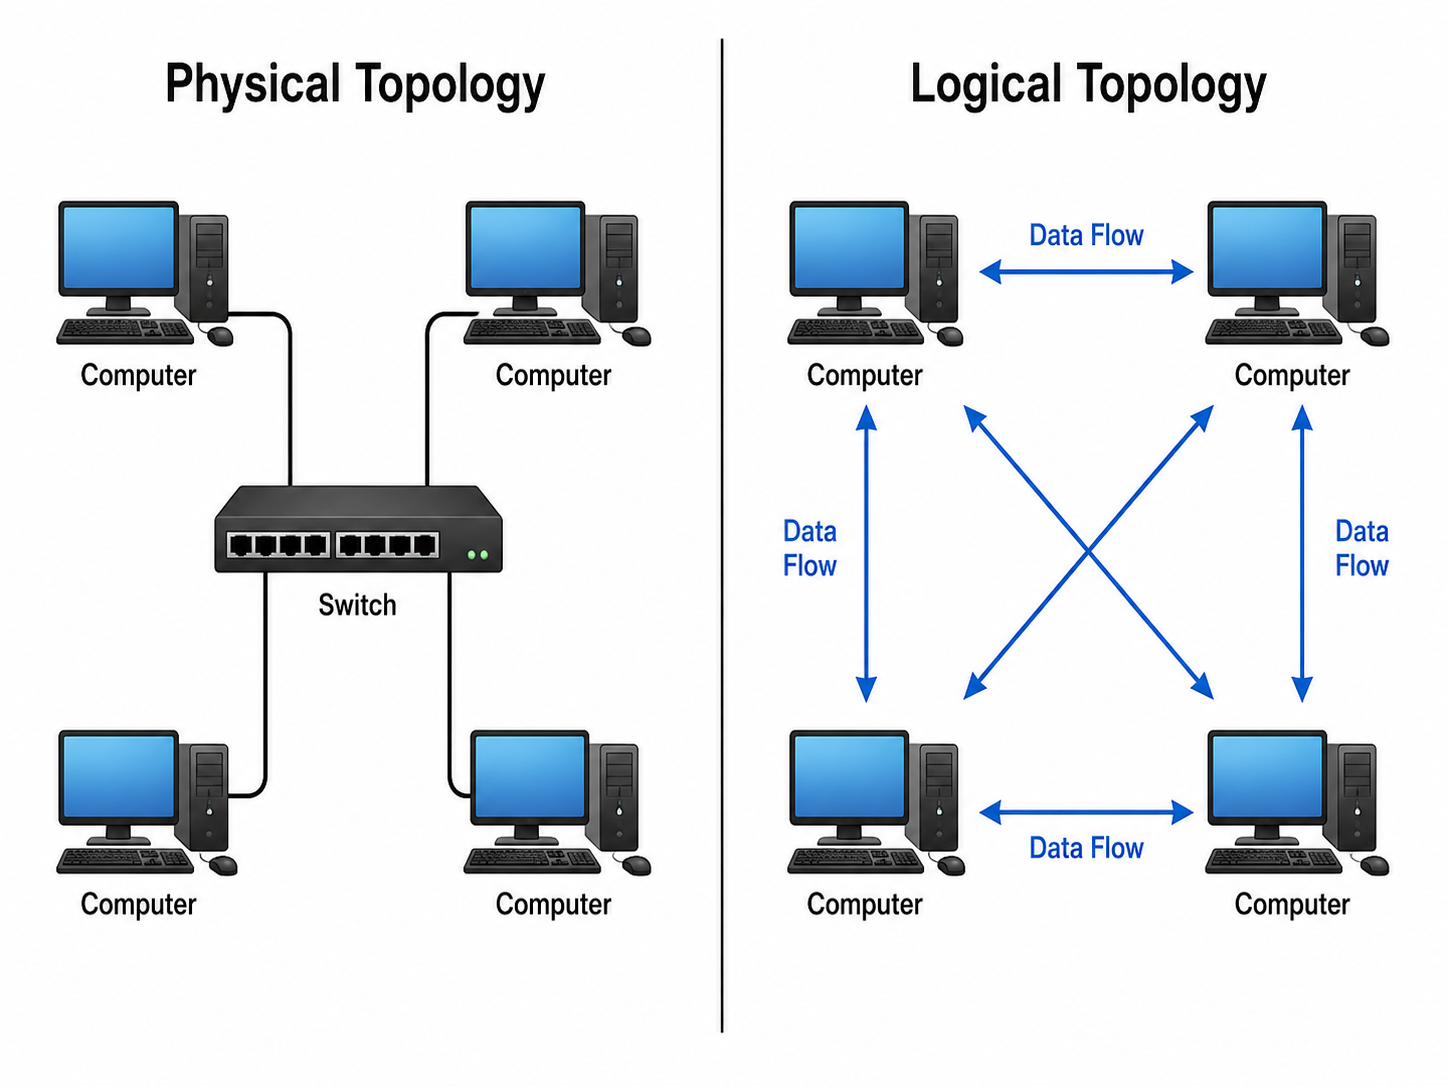
\includegraphics[width=0.92\textwidth]{chapters/Chapter02/images/physical_vs_logical_topology.png}
}{
\fbox{
\parbox{0.90\textwidth}{
\centering
\vspace{0.7cm}
Physical Topology: Actual device and cable layout[8pt]
Logical Topology: Data flow path
\vspace{0.7cm}
}}
}
\caption{Physical topology ও Logical topology}
\end{figure}

\subsection{নেটওয়ার্ক টপোলজির প্রকারভেদ}

HSC ICT-তে নিচের topology-গুলো সবচেয়ে গুরুত্বপূর্ণ:

\begin{itemize}
\item Bus Topology
\item Star Topology
\item Ring Topology
\item Mesh Topology
\item Tree Topology
\item Hybrid Topology
\end{itemize}

\begin{figure}[H]
\centering
\IfFileExists{chapters/Chapter02/images/network_topology_classification_tree.png}{
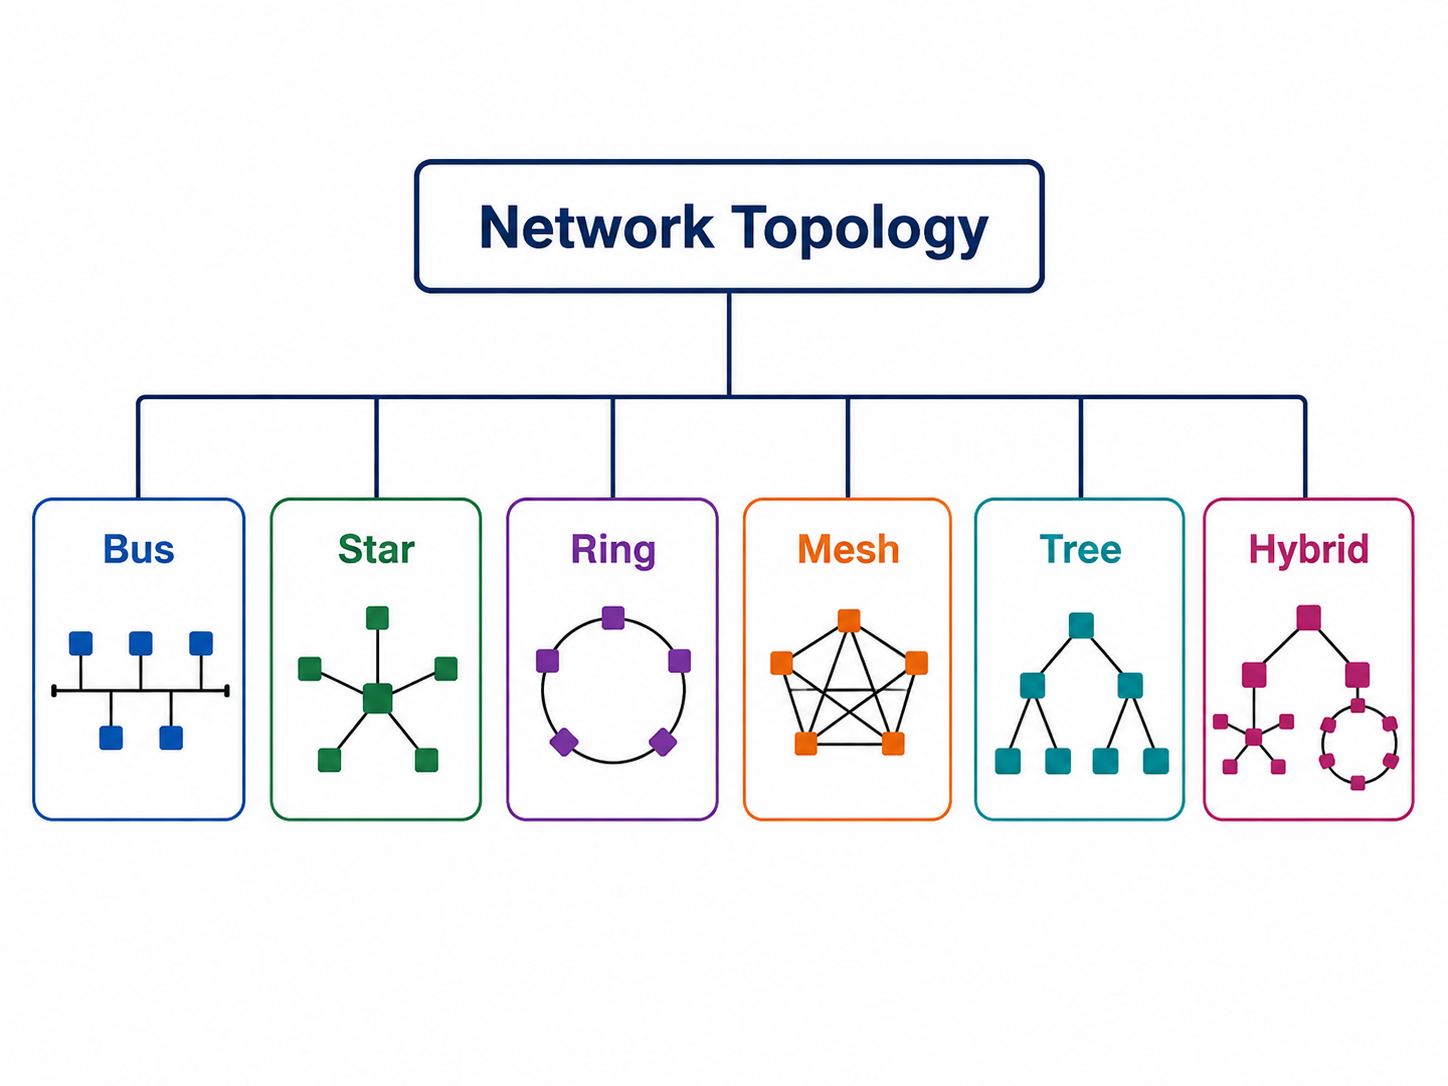
\includegraphics[width=0.92\textwidth]{chapters/Chapter02/images/network_topology_classification_tree.png}
}{
\fbox{
\parbox{0.90\textwidth}{
\centering
\vspace{0.7cm}
Network Topology[8pt]
Bus \quad Star \quad Ring \quad Mesh \quad Tree \quad Hybrid
\vspace{0.7cm}
}}
}
\caption{নেটওয়ার্ক টপোলজির প্রকারভেদ}
\end{figure}

\subsection{Bus Topology}

\begin{definitionbox}{Bus Topology}
যে network topology-তে সব node একটি common communication line বা backbone cable-এর সাথে যুক্ত থাকে, তাকে Bus topology বলা হয়।
\end{definitionbox}

Bus topology-তে একটি main cable বা backbone থাকে। সব computer বা node এই backbone cable-এর সাথে connected থাকে। কোনো node data পাঠালে data backbone cable দিয়ে travel করে এবং destination node সেটি গ্রহণ করে।

\begin{keypointbox}{Bus topology-এর বৈশিষ্ট্য}
\begin{itemize}
\item একটি main backbone cable থাকে।
\item সব node একই cable-এর সাথে connected থাকে।
\item installation তুলনামূলক সহজ।
\item cable কম লাগে, তাই cost কম হতে পারে।
\item backbone cable নষ্ট হলে পুরো network বন্ধ হতে পারে।
\item বেশি node যুক্ত হলে performance কমে যেতে পারে।
\item troubleshooting তুলনামূলক কঠিন হতে পারে।
\end{itemize}
\end{keypointbox}

\begin{figure}[H]
\centering
\IfFileExists{chapters/Chapter02/images/bus_topology_diagram.png}{
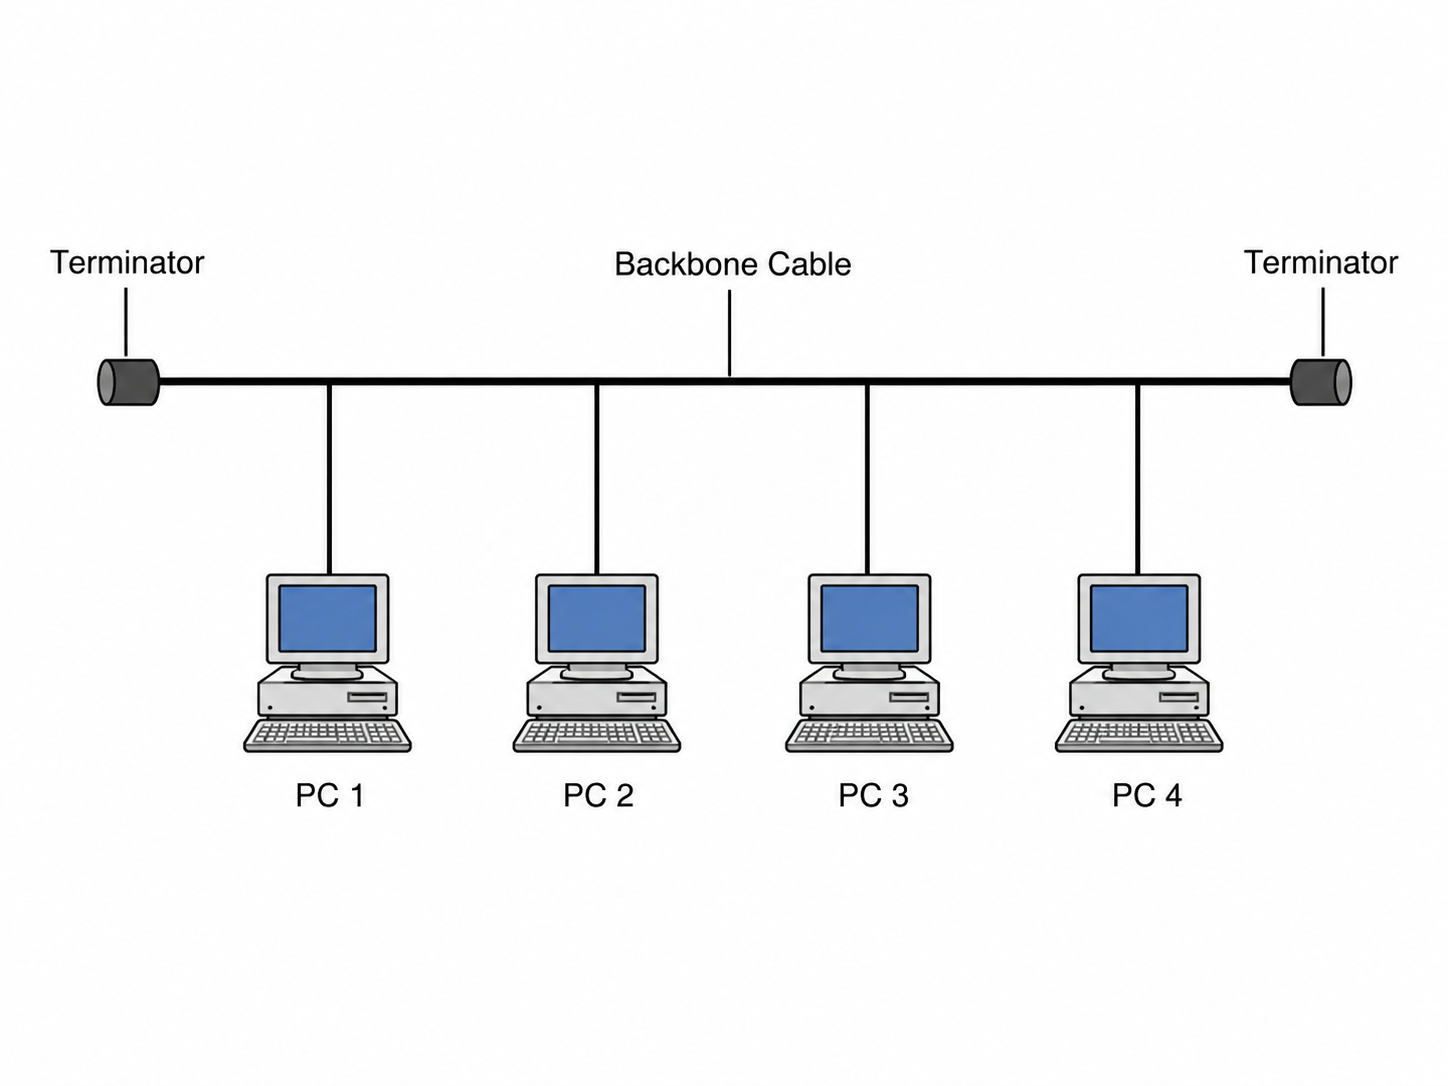
\includegraphics[width=0.92\textwidth]{chapters/Chapter02/images/bus_topology_diagram.png}
}{
\fbox{
\parbox{0.90\textwidth}{
\centering
\vspace{0.7cm}
PC 1 \quad PC 2 \quad PC 3 \quad PC 4[6pt]
\rule{0.75\textwidth}{1pt}[6pt]
Backbone Cable
\vspace{0.7cm}
}}
}
\caption{Bus topology}
\end{figure}

\begin{examplebox}{বাস্তব উদাহরণ}
পুরনো Ethernet network-এ coaxial cable ব্যবহার করে Bus topology দেখা যেত। ছোট বা temporary network design বোঝাতে এই topology ব্যবহার করা হয়।
\end{examplebox}

\begin{boardbox}{বোর্ড ফোকাস}
Bus topology-এর উত্তরে অবশ্যই “সব node একটি common backbone cable-এর সাথে যুক্ত থাকে” কথাটি লিখবে। Backbone cable failure হলে পুরো network প্রভাবিত হয়—এটি গুরুত্বপূর্ণ point।
\end{boardbox}

\subsection{Bus Topology-এর সুবিধা ও অসুবিধা}

\begin{center}
\begin{tabular}{|p{0.43\textwidth}|p{0.43\textwidth}|}
\hline
\textbf{সুবিধা} & \textbf{অসুবিধা} \
\hline
cable কম লাগে & backbone cable নষ্ট হলে network বন্ধ হতে পারে \
\hline
cost তুলনামূলক কম & বেশি node হলে traffic বাড়ে \
\hline
ছোট network-এ setup সহজ & fault খুঁজে বের করা কঠিন \
\hline
অস্থায়ী network-এর জন্য ব্যবহারযোগ্য & security ও performance তুলনামূলক কম \
\hline
\end{tabular}
\end{center}

\subsection{Star Topology}

\begin{definitionbox}{Star Topology}
যে network topology-তে সব node একটি central device যেমন switch বা hub-এর সাথে আলাদাভাবে connected থাকে, তাকে Star topology বলা হয়।
\end{definitionbox}

Star topology আধুনিক LAN-এ সবচেয়ে বেশি ব্যবহৃত topology-এর একটি। এখানে প্রতিটি computer আলাদা cable দ্বারা central switch বা hub-এর সাথে connected থাকে। কোনো একটি node-এর cable নষ্ট হলে সাধারণত শুধু সেই node affected হয়, পুরো network নয়। তবে central device নষ্ট হলে পুরো network প্রভাবিত হতে পারে।

\begin{keypointbox}{Star topology-এর বৈশিষ্ট্য}
\begin{itemize}
\item একটি central device থাকে।
\item প্রতিটি node central device-এর সাথে আলাদা link দিয়ে যুক্ত।
\item নতুন node add করা সহজ।
\item troubleshooting তুলনামূলক সহজ।
\item একটি node বা cable failure হলে পুরো network সাধারণত বন্ধ হয় না।
\item central device failure হলে network বন্ধ হতে পারে।
\item cable requirement bus topology-এর তুলনায় বেশি হতে পারে।
\end{itemize}
\end{keypointbox}

\begin{figure}[H]
\centering
\IfFileExists{chapters/Chapter02/images/star_topology_diagram.png}{
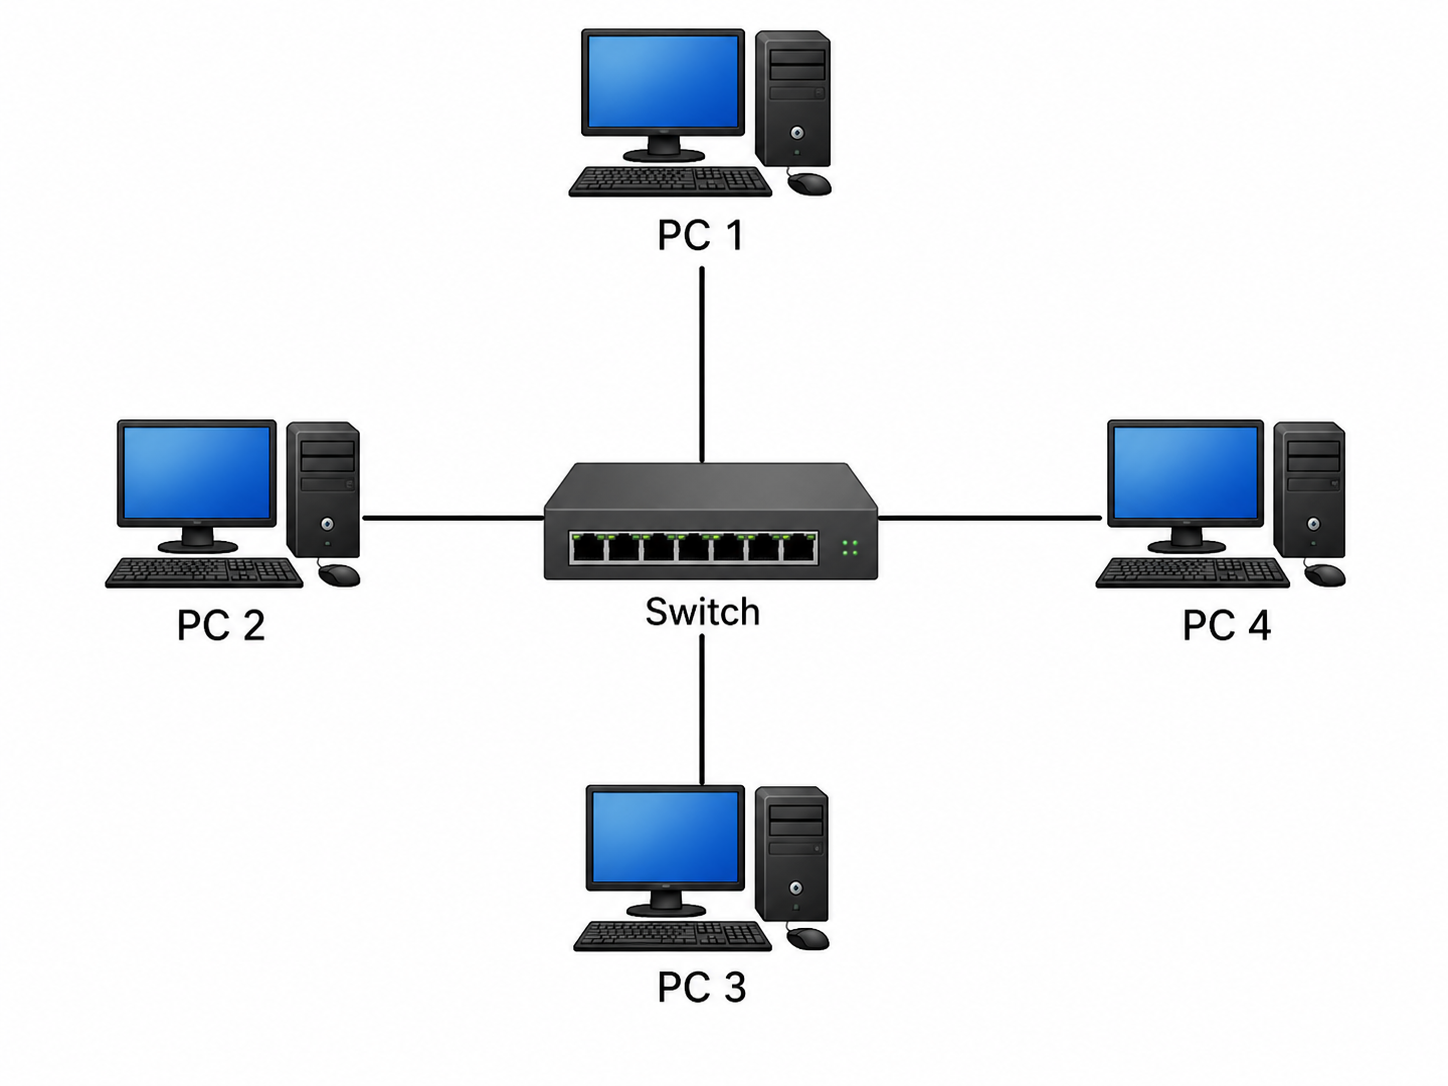
\includegraphics[width=0.86\textwidth]{chapters/Chapter02/images/star_topology_diagram.png}
}{
\fbox{
\parbox{0.84\textwidth}{
\centering
\vspace{0.7cm}
PC 1 \quad \quad PC 2[8pt]
\quad \diagdown \quad \quad \diagup[4pt]
\quad Switch / Hub[4pt]
\quad \diagup \quad \quad \diagdown[8pt]
PC 3 \quad \quad PC 4
\vspace{0.7cm}
}}
}
\caption{Star topology}
\end{figure}

\begin{examplebox}{বাস্তব উদাহরণ}
School computer lab বা office LAN-এ সাধারণত সব computer একটি switch-এর সাথে connected থাকে। এটি Star topology-এর বাস্তব উদাহরণ।
\end{examplebox}

\begin{boardbox}{বোর্ড ফোকাস}
Star topology-এর উত্তরে “central device” বা “switch/hub” উল্লেখ করা জরুরি। এটি আধুনিক LAN-এর জন্য খুব common topology।
\end{boardbox}

\subsection{Star Topology-এর সুবিধা ও অসুবিধা}

\begin{center}
\begin{tabular}{|p{0.43\textwidth}|p{0.43\textwidth}|}
\hline
\textbf{সুবিধা} & \textbf{অসুবিধা} \
\hline
installation ও management সহজ & central device নষ্ট হলে network বন্ধ হতে পারে \
\hline
নতুন node add করা সহজ & cable বেশি লাগে \
\hline
fault finding সহজ & central device-এর cost থাকে \
\hline
এক node failure পুরো network বন্ধ করে না & central device-এর উপর dependency বেশি \
\hline
performance ভালো হতে পারে, বিশেষ করে switch ব্যবহারে & বড় network-এ ভালো device দরকার \
\hline
\end{tabular}
\end{center}

\subsection{Ring Topology}

\begin{definitionbox}{Ring Topology}
যে network topology-তে প্রতিটি node তার পাশের দুইটি node-এর সাথে connected থাকে এবং সব node মিলে একটি closed loop বা ring তৈরি করে, তাকে Ring topology বলা হয়।
\end{definitionbox}

Ring topology-তে data সাধারণত একটি নির্দিষ্ট direction-এ node থেকে node-এ travel করে। একটি node data receive করে দেখে সেটি তার জন্য কি না। যদি তার জন্য না হয়, তাহলে পরবর্তী node-এ forward করে।

\begin{keypointbox}{Ring topology-এর বৈশিষ্ট্য}
\begin{itemize}
\item node-গুলো ring বা closed loop আকারে connected থাকে।
\item প্রতিটি node সাধারণত দুইটি neighboring node-এর সাথে যুক্ত থাকে।
\item data এক direction বা নির্দিষ্ট path ধরে travel করতে পারে।
\item collision কম হতে পারে।
\item কোনো node বা link failure হলে network প্রভাবিত হতে পারে।
\item troubleshooting তুলনামূলক জটিল হতে পারে।
\end{itemize}
\end{keypointbox}

\begin{figure}[H]
\centering
\IfFileExists{chapters/Chapter02/images/ring_topology_diagram.png}{
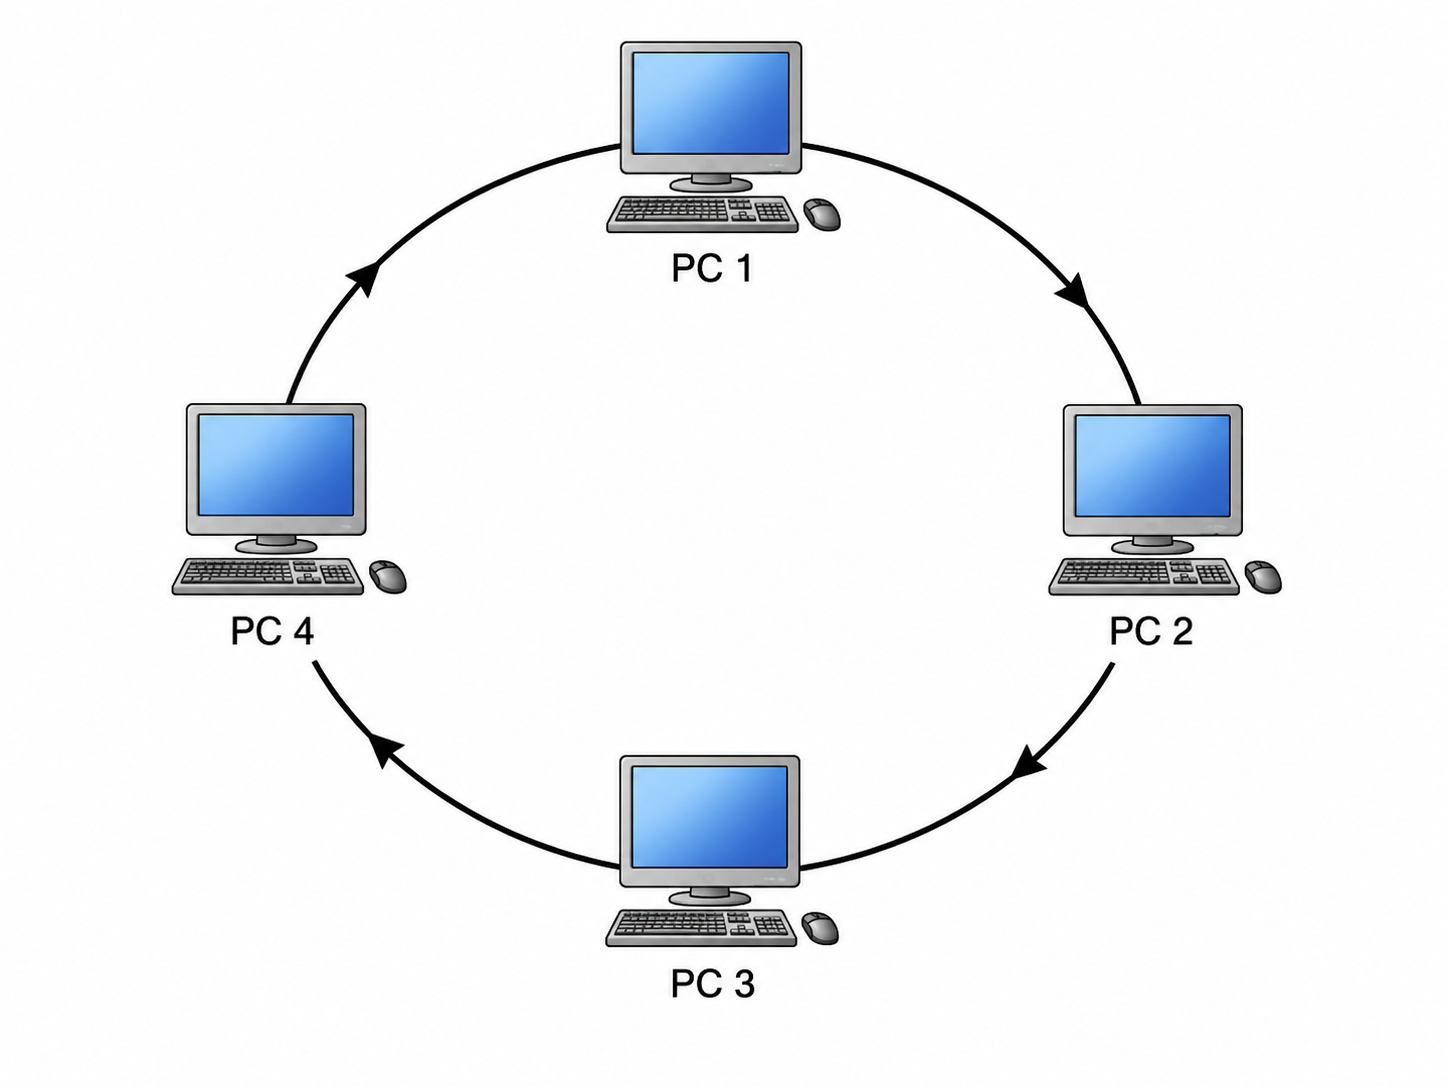
\includegraphics[width=0.86\textwidth]{chapters/Chapter02/images/ring_topology_diagram.png}
}{
\fbox{
\parbox{0.84\textwidth}{
\centering
\vspace{0.7cm}
PC 1 \quad $\longrightarrow$ \quad PC 2[8pt]
$\uparrow$ \qquad \qquad \qquad $\downarrow$[8pt]
PC 4 \quad $\longleftarrow$ \quad PC 3[8pt]
Closed Loop
\vspace{0.7cm}
}}
}
\caption{Ring topology}
\end{figure}

\begin{examplebox}{সহজ উদাহরণ}
যদি চারটি computer এমনভাবে connected থাকে যে PC1 থেকে PC2, PC2 থেকে PC3, PC3 থেকে PC4 এবং PC4 আবার PC1-এর সাথে connected, তাহলে এটি Ring topology।
\end{examplebox}

\subsection{Ring Topology-এর সুবিধা ও অসুবিধা}

\begin{center}
\begin{tabular}{|p{0.43\textwidth}|p{0.43\textwidth}|}
\hline
\textbf{সুবিধা} & \textbf{অসুবিধা} \
\hline
data নির্দিষ্ট path ধরে flow করে & একটি node/link failure network প্রভাবিত করতে পারে \
\hline
collision কম হতে পারে & troubleshooting কঠিন \
\hline
traffic predictable হতে পারে & নতুন node add করা তুলনামূলক কঠিন \
\hline
small controlled network-এ ব্যবহারযোগ্য & delay বাড়তে পারে কারণ data এক node থেকে অন্য node-এ যায় \
\hline
\end{tabular}
\end{center}

\subsection{Mesh Topology}

\begin{definitionbox}{Mesh Topology}
যে network topology-তে প্রতিটি node অন্য node-গুলোর সাথে সরাসরি বা একাধিক path দ্বারা connected থাকে, তাকে Mesh topology বলা হয়।
\end{definitionbox}

Mesh topology দুই ধরনের হতে পারে:

\begin{itemize}
\item \textbf{Full Mesh}: প্রতিটি node অন্য প্রতিটি node-এর সাথে সরাসরি connected।
\item \textbf{Partial Mesh}: সব node নয়, কিছু গুরুত্বপূর্ণ node একাধিক link দিয়ে connected।
\end{itemize}

Mesh topology অত্যন্ত reliable, কারণ একটি link নষ্ট হলেও alternative path দিয়ে data যেতে পারে। তবে বেশি cable, বেশি port এবং বেশি cost দরকার হয়।

\begin{keypointbox}{Mesh topology-এর বৈশিষ্ট্য}
\begin{itemize}
\item multiple path থাকে।
\item reliability বেশি।
\item fault tolerance ভালো।
\item security তুলনামূলক বেশি হতে পারে, কারণ dedicated link থাকতে পারে।
\item installation ও maintenance complex।
\item cable ও device port বেশি লাগে।
\item বড় backbone বা critical network-এ mesh concept গুরুত্বপূর্ণ।
\end{itemize}
\end{keypointbox}

\begin{figure}[H]
\centering
\IfFileExists{chapters/Chapter02/images/mesh_topology_diagram.png}{
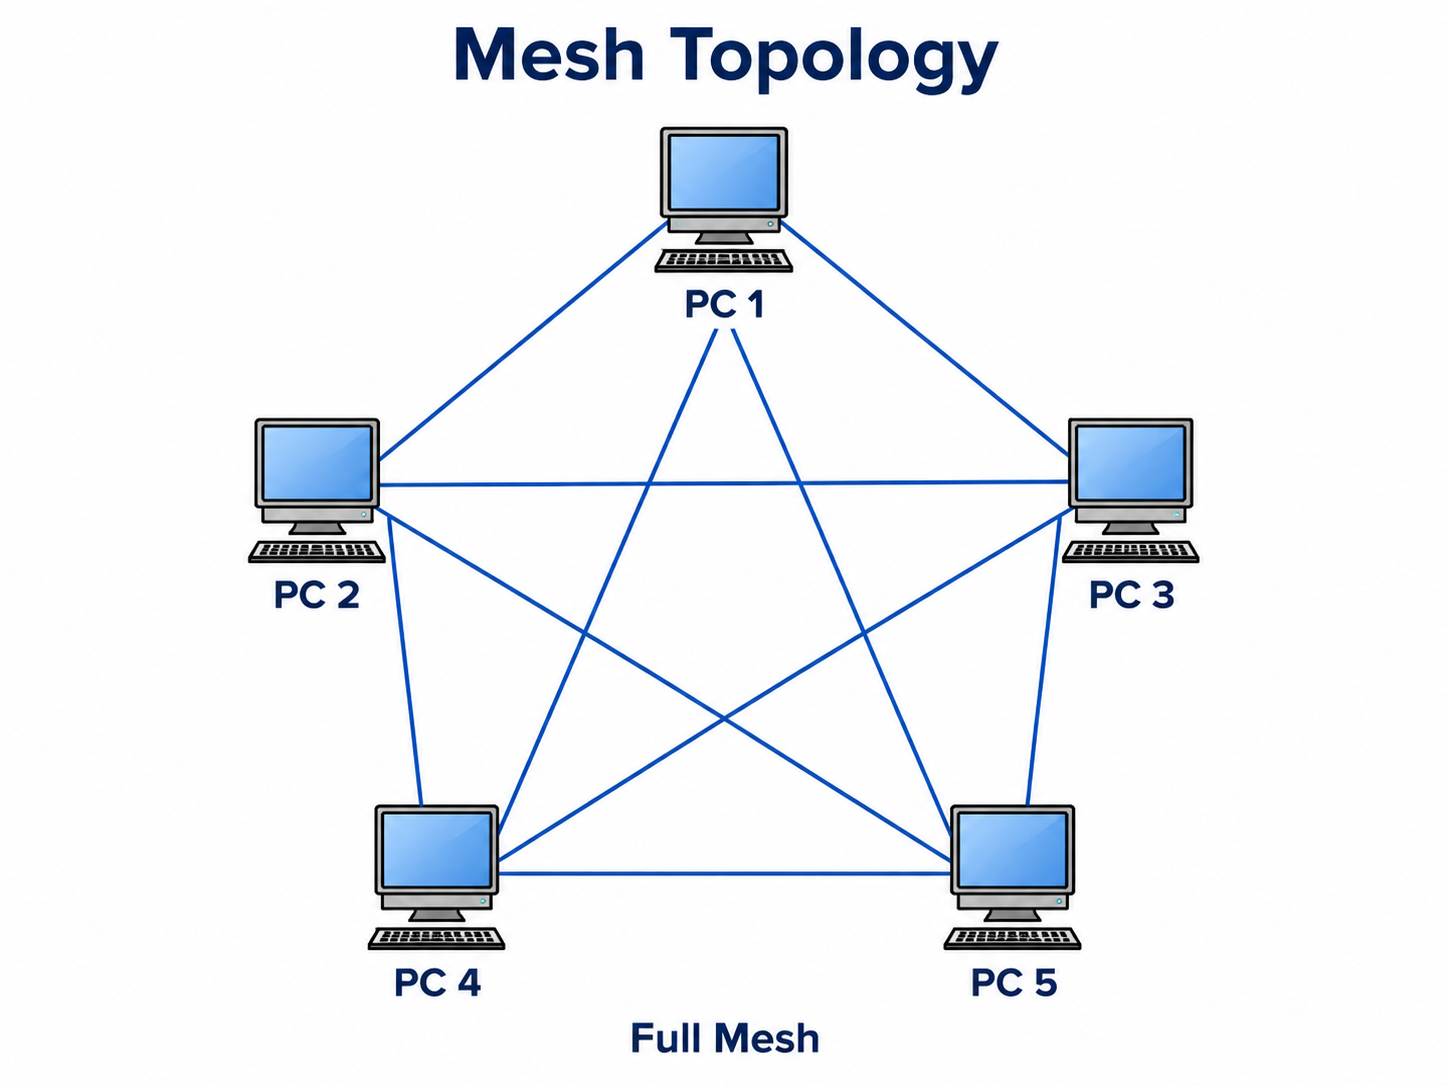
\includegraphics[width=0.86\textwidth]{chapters/Chapter02/images/mesh_topology_diagram.png}
}{
\fbox{
\parbox{0.84\textwidth}{
\centering
\vspace{0.7cm}
PC 1 \quad \rule{2cm}{0.5pt} \quad PC 2[8pt]
|\diagdown \quad \diagup|[8pt]
|\diagup \quad \diagdown|[8pt]
PC 3 \quad \rule{2cm}{0.5pt} \quad PC 4[8pt]
Multiple Links
\vspace{0.7cm}
}}
}
\caption{Mesh topology}
\end{figure}

\begin{examplebox}{বাস্তব উদাহরণ}
High reliability দরকার এমন network, যেমন backbone network, military communication বা critical data center interconnection-এ mesh বা partial mesh design ব্যবহার করা যেতে পারে।
\end{examplebox}

\subsection{Mesh Topology-এর সুবিধা ও অসুবিধা}

\begin{center}
\begin{tabular}{|p{0.43\textwidth}|p{0.43\textwidth}|}
\hline
\textbf{সুবিধা} & \textbf{অসুবিধা} \
\hline
reliability খুব বেশি & cable ও port বেশি লাগে \
\hline
alternative path থাকে & installation cost বেশি \
\hline
fault tolerance ভালো & design ও maintenance complex \
\hline
এক link নষ্ট হলেও communication চলতে পারে & ছোট সাধারণ network-এর জন্য অতিরিক্ত ব্যয়বহুল \
\hline
\end{tabular}
\end{center}

\subsection{Tree Topology}

\begin{definitionbox}{Tree Topology}
যে topology-তে star topology-এর একাধিক group hierarchy বা tree structure আকারে connected থাকে, তাকে Tree topology বলা হয়।
\end{definitionbox}

Tree topology-তে root বা backbone level থাকে এবং তার নিচে branch আকারে বিভিন্ন star network connected থাকতে পারে। বড় school, college, office বা campus network বোঝাতে Tree topology useful।

\begin{keypointbox}{Tree topology-এর বৈশিষ্ট্য}
\begin{itemize}
\item hierarchical structure থাকে।
\item একাধিক star topology combine হতে পারে।
\item বড় network organize করা সহজ।
\item department বা floor-wise network design করা যায়।
\item backbone বা root device নষ্ট হলে বড় অংশ affected হতে পারে।
\item cable ও device planning দরকার হয়।
\end{itemize}
\end{keypointbox}

\begin{figure}[H]
\centering
\IfFileExists{chapters/Chapter02/images/tree_topology_diagram.png}{
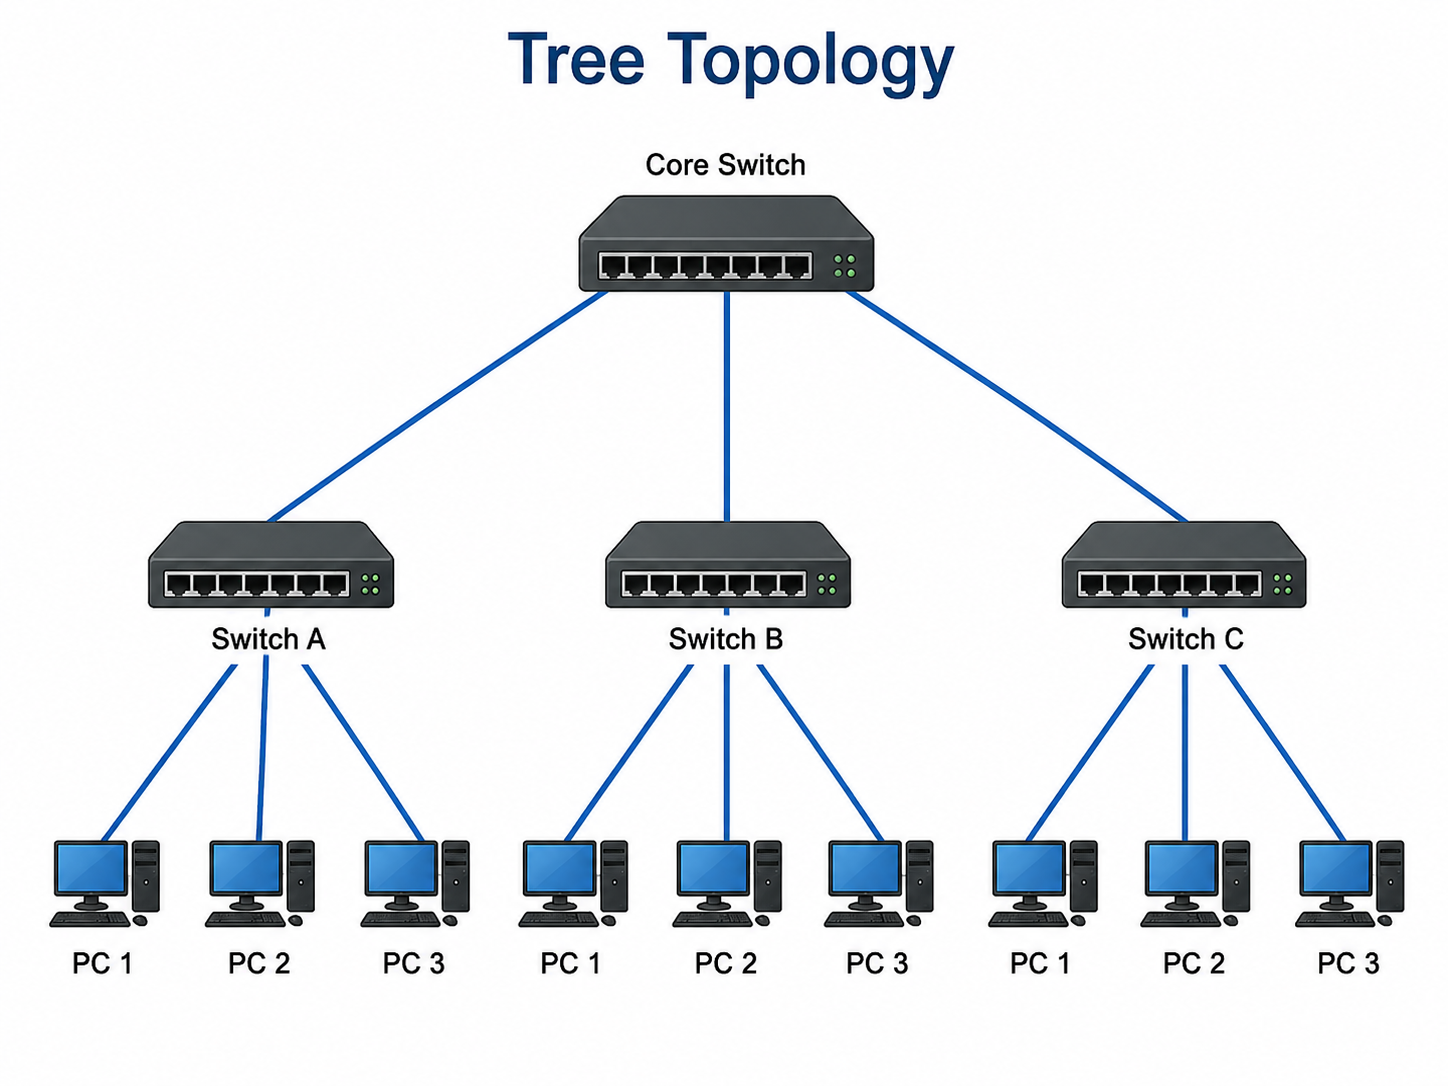
\includegraphics[width=0.90\textwidth]{chapters/Chapter02/images/tree_topology_diagram.png}
}{
\fbox{
\parbox{0.88\textwidth}{
\centering
\vspace{0.7cm}
Core Switch[8pt]
$\swarrow$ \quad $\downarrow$ \quad $\searrow$[8pt]
Switch A \quad Switch B \quad Switch C[8pt]
$\downarrow$ \quad \quad $\downarrow$ \quad \quad $\downarrow$[8pt]
PC Group A \quad PC Group B \quad PC Group C
\vspace{0.7cm}
}}
}
\caption{Tree topology}
\end{figure}

\begin{examplebox}{বাস্তব উদাহরণ}
একটি কলেজের admin building, ICT lab ও library-এর network আলাদা switch-এ connected, আর সব switch একটি core switch-এর সাথে connected—এটি Tree topology দিয়ে বোঝানো যায়।
\end{examplebox}

\subsection{Tree Topology-এর সুবিধা ও অসুবিধা}

\begin{center}
\begin{tabular}{|p{0.43\textwidth}|p{0.43\textwidth}|}
\hline
	\textbf{সুবিধা} & \textbf{অসুবিধা} \\
\hline
বড় network manage করা সহজ & backbone/root failure বড় অংশকে প্রভাবিত করতে পারে \\
\hline
department-wise network করা যায় & cable ও device বেশি লাগে \\
\hline
scalable, অর্থাৎ node add করা সহজ & configuration ও maintenance complex হতে পারে \\
\hline
fault isolation কিছুটা সহজ & cost তুলনামূলক বেশি \\
\hline
\end{tabular}
\end{center}

\subsection{Hybrid Topology}

\begin{definitionbox}{Hybrid Topology}
দুই বা ততোধিক topology একত্রে ব্যবহার করে যে network topology তৈরি হয়, তাকে Hybrid topology বলা হয়।
\end{definitionbox}

বাস্তব বড় network-এ অনেক সময় একটি topology যথেষ্ট হয় না। যেমন একটি campus network-এ computer lab-এ Star topology, building-to-building connection-এ Mesh/Tree concept এবং wireless area-তে access point-based star structure থাকতে পারে। এই combination-ই Hybrid topology।

\begin{keypointbox}{Hybrid topology-এর বৈশিষ্ট্য}
\begin{itemize}
\item একাধিক topology combine করে তৈরি হয়।
\item বাস্তব বড় network design-এ বেশি ব্যবহারযোগ্য।
\item flexibility বেশি।
\item performance ও reliability requirement অনুযায়ী design করা যায়।
\item design, installation ও maintenance complex।
\item cost তুলনামূলক বেশি হতে পারে।
\end{itemize}
\end{keypointbox}

\begin{figure}[H]
\centering
\IfFileExists{chapters/Chapter02/images/hybrid_topology_diagram.png}{
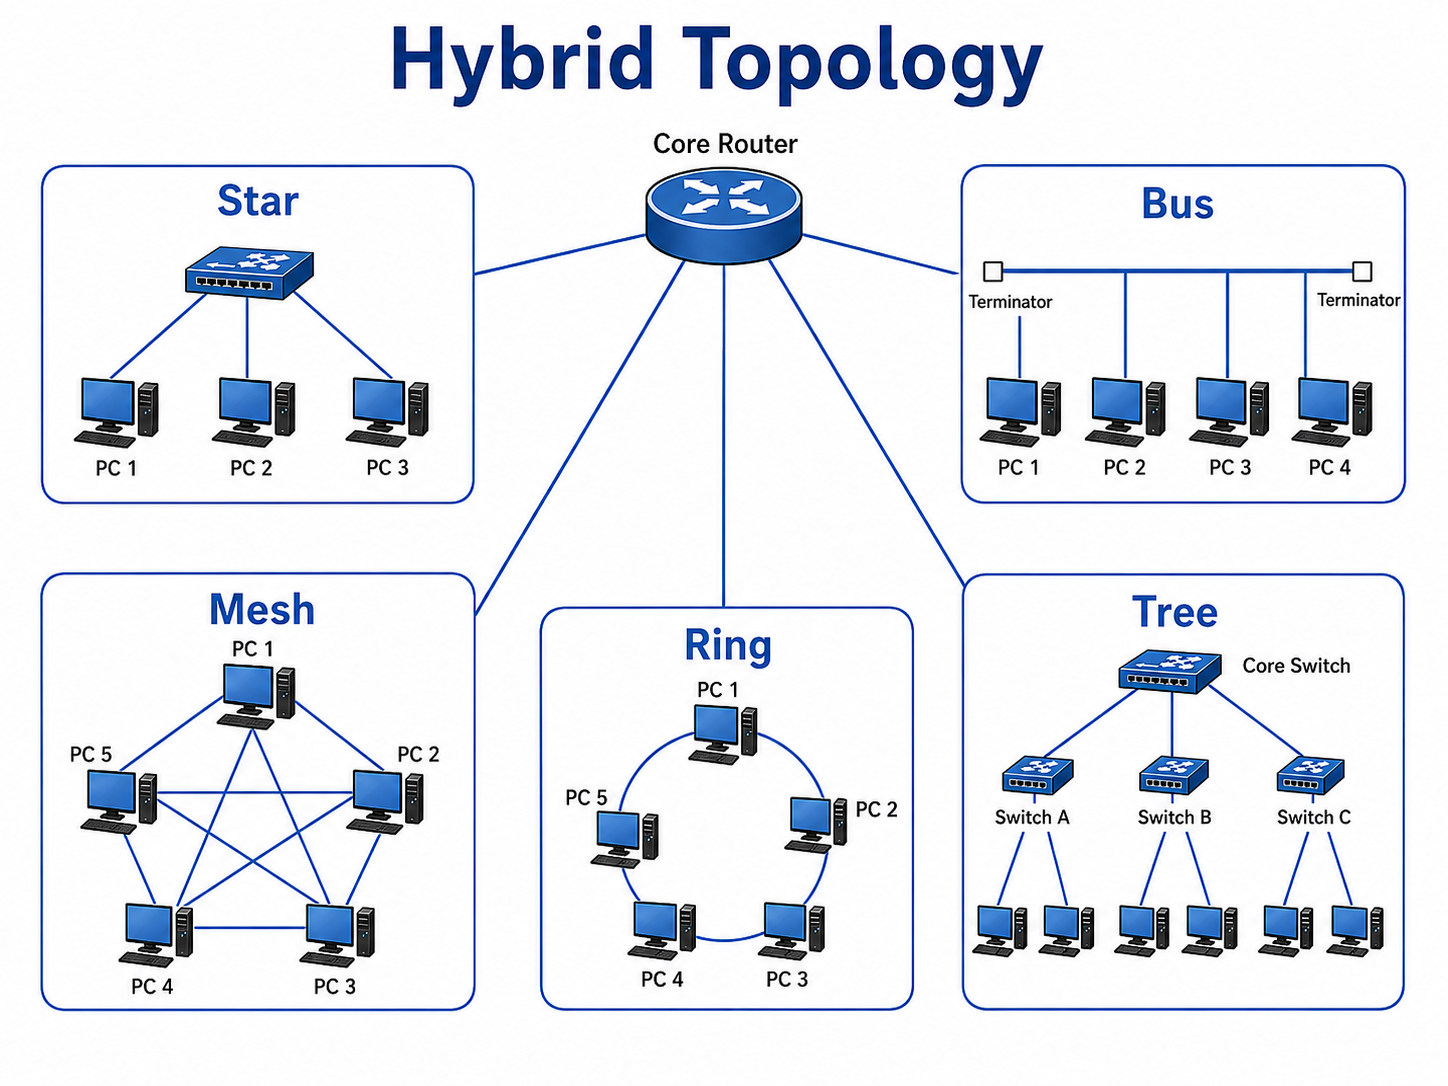
\includegraphics[width=0.92\textwidth]{chapters/Chapter02/images/hybrid_topology_diagram.png}
}{
\fbox{
\parbox{0.90\textwidth}{
\centering
\vspace{0.7cm}
Star Group A \quad $\longleftrightarrow$ \quad Core Router/Switch \quad $\longleftrightarrow$ \quad Star Group B[8pt]
Mesh/Tree Backbone + Star LAN Groups
\vspace{0.7cm}
}}
}
\caption{Hybrid topology}
\end{figure}

\begin{examplebox}{বাস্তব উদাহরণ}
একটি university campus network-এ প্রতিটি department star topology ব্যবহার করতে পারে, আবার department switches গুলো core network-এর সাথে tree/hybrid structure-এ connected থাকতে পারে।
\end{examplebox}

\subsection{প্রধান Topology-গুলোর তুলনা}

\begin{center}
\begin{tabular}{|p{0.16\textwidth}|p{0.23\textwidth}|p{0.22\textwidth}|p{0.22\textwidth}|}
\hline
\textbf{Topology} & \textbf{Structure} & \textbf{সুবিধা} & \textbf{অসুবিধা} \
\hline
Bus & common backbone cable & cost কম, সহজ setup & backbone failure-এ network বন্ধ \
\hline
Star & central switch/hub & manage ও troubleshoot সহজ & central device failure risky \
\hline
Ring & closed loop & ordered data flow & node/link failure problem \
\hline
Mesh & multiple interconnection & reliability বেশি & cost ও complexity বেশি \
\hline
Tree & hierarchical structure & বড় network organize সহজ & backbone/root dependency \
\hline
Hybrid & mixed topology & flexible ও practical & design complex, cost বেশি \
\hline
\end{tabular}
\end{center}

\begin{figure}[H]
\centering
\IfFileExists{chapters/Chapter02/images/network_topology_comparison_chart.png}{
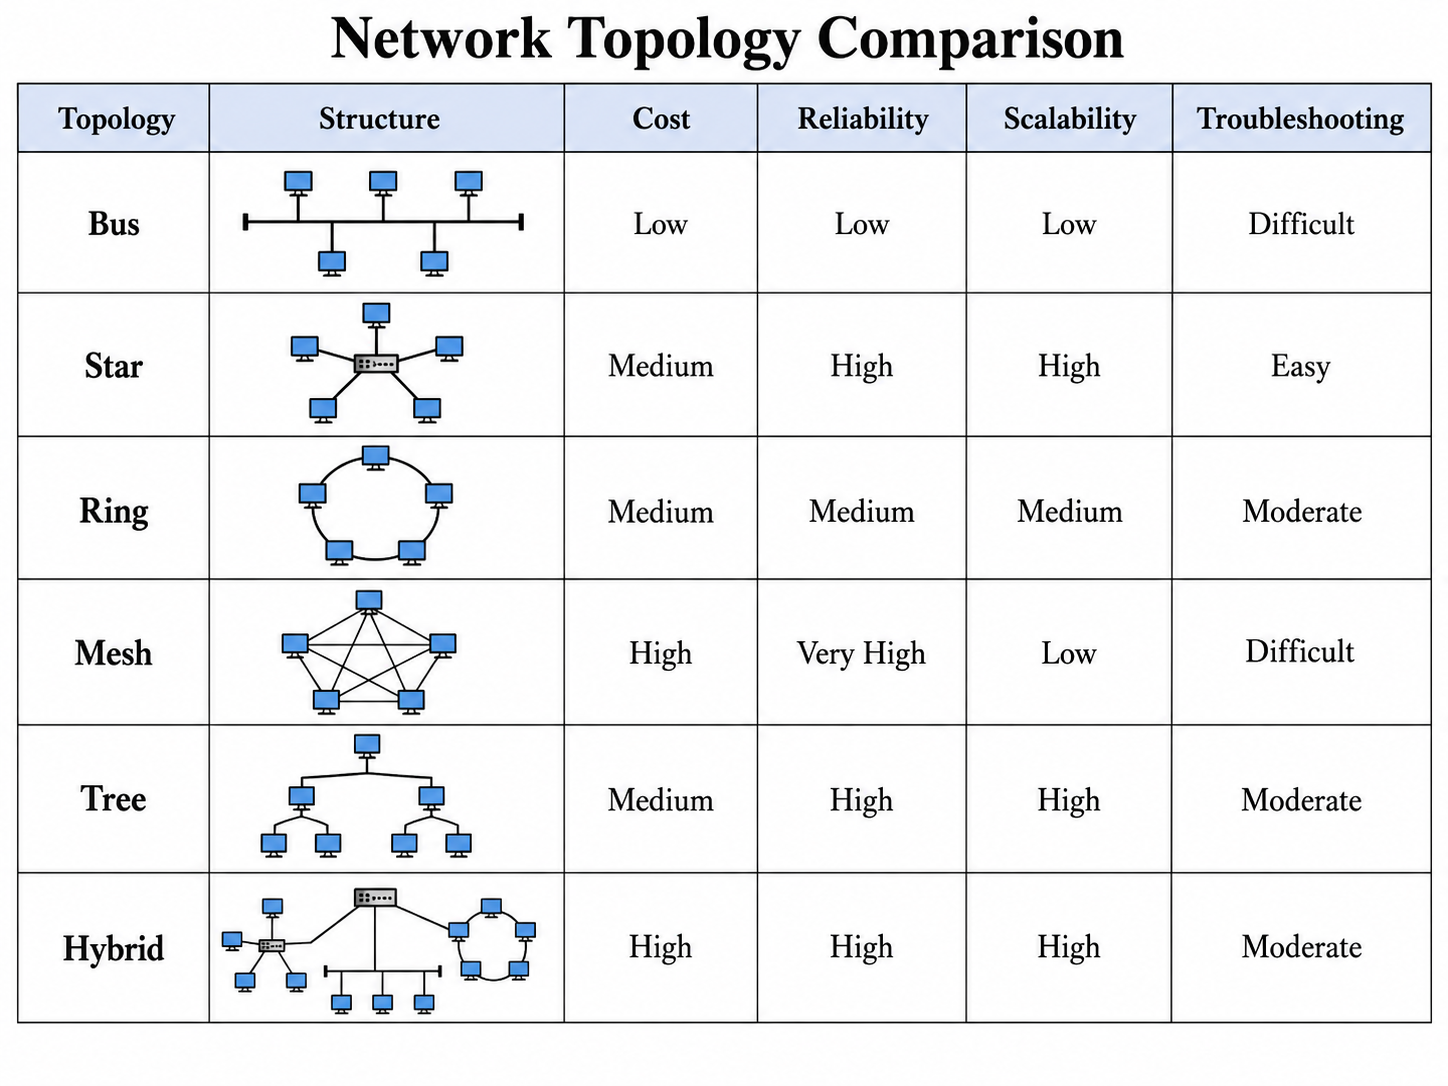
\includegraphics[width=0.94\textwidth]{chapters/Chapter02/images/network_topology_comparison_chart.png}
}{
\fbox{
\parbox{0.92\textwidth}{
\centering
\vspace{0.7cm}
Bus \quad Star \quad Ring \quad Mesh \quad Tree \quad Hybrid[8pt]
Cost \quad Reliability \quad Scalability \quad Troubleshooting
\vspace{0.7cm}
}}
}
\caption{নেটওয়ার্ক টপোলজির তুলনা}
\end{figure}

\subsection{কোন পরিস্থিতিতে কোন topology ব্যবহার হবে?}

\begin{center}
\begin{tabular}{|p{0.34\textwidth}|p{0.24\textwidth}|p{0.30\textwidth}|}
\hline
\textbf{পরিস্থিতি} & \textbf{উপযুক্ত topology} & \textbf{কারণ} \
\hline
ছোট পুরনো বা temporary network & Bus & cable কম লাগে, setup সহজ \
\hline
School computer lab & Star & switch দিয়ে device manage সহজ \
\hline
ordered data flow দরকার এমন controlled network & Ring & data নির্দিষ্ট path ধরে যায় \
\hline
high reliability critical network & Mesh & alternative path থাকে \
\hline
বড় office বা campus network & Tree & hierarchy অনুযায়ী network organize করা যায় \
\hline
university/corporate mixed network & Hybrid & বিভিন্ন requirement অনুযায়ী topology mix করা যায় \
\hline
\end{tabular}
\end{center}

\begin{figure}[H]
\centering
\IfFileExists{chapters/Chapter02/images/topology_selection_scenario.png}{
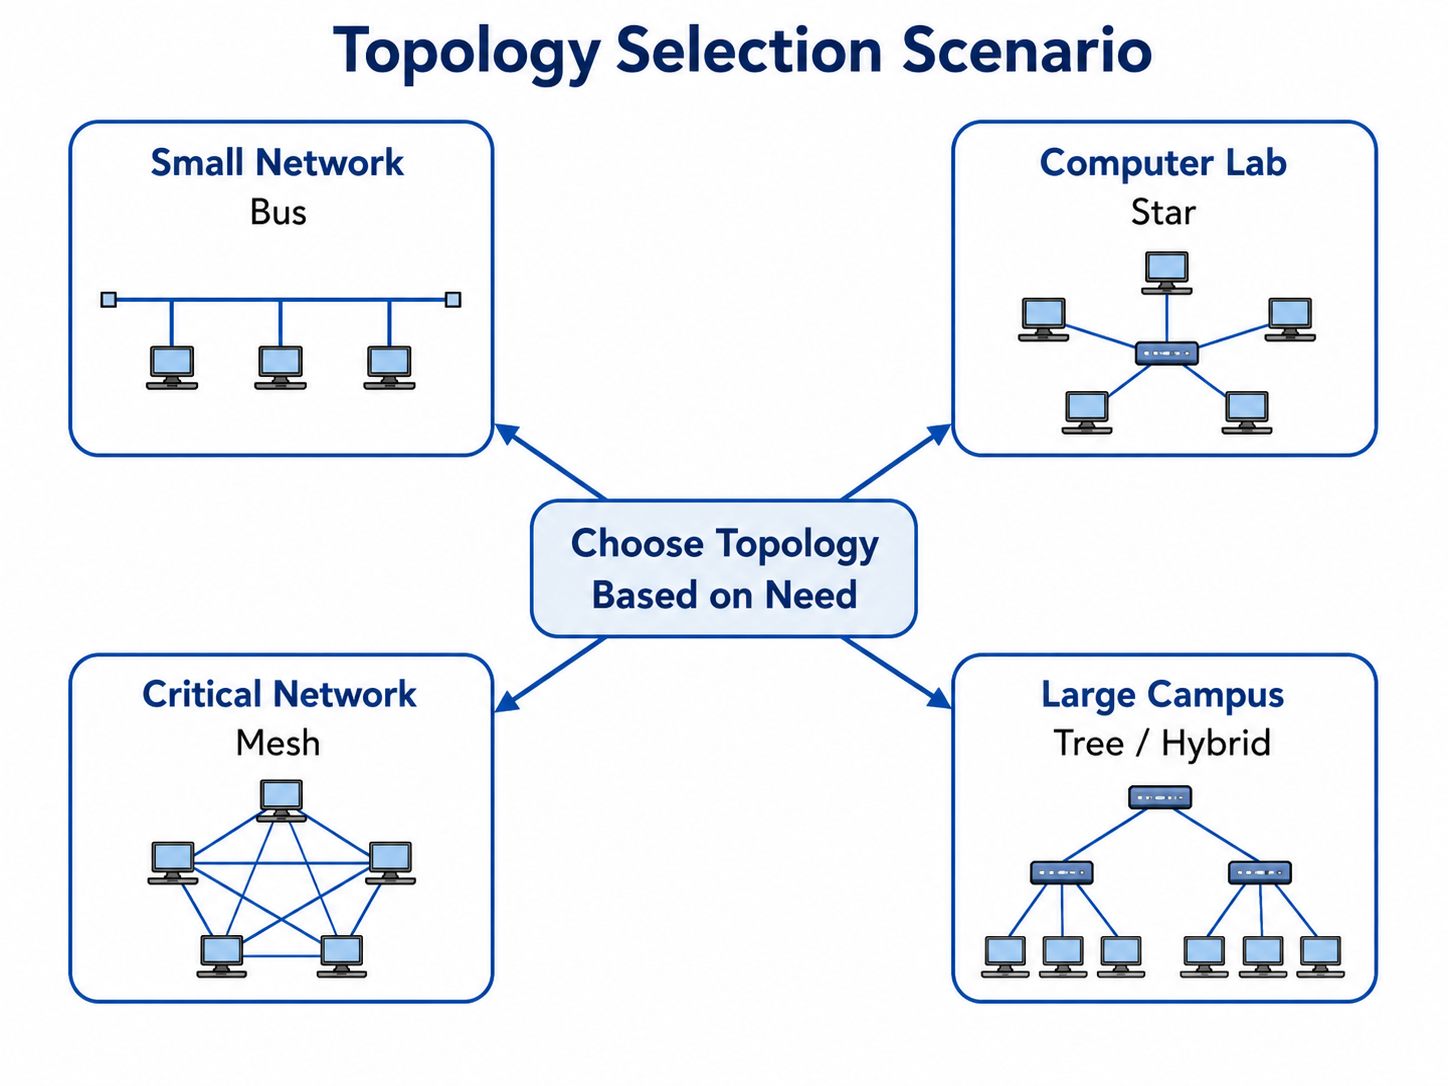
\includegraphics[width=0.92\textwidth]{chapters/Chapter02/images/topology_selection_scenario.png}
}{
\fbox{
\parbox{0.90\textwidth}{
\centering
\vspace{0.7cm}
Small Lab: Star[6pt]
Campus: Tree / Hybrid[6pt]
Critical Backbone: Mesh[6pt]
Temporary Network: Bus
\vspace{0.7cm}
}}
}
\caption{পরিস্থিতি অনুযায়ী topology নির্বাচন}
\end{figure}

\subsection{Topology নির্বাচন করার সময় বিবেচ্য বিষয়}

সব network-এর জন্য একই topology best নয়। ব্যবহার, budget, reliability, security, future expansion এবং maintenance facility অনুযায়ী topology নির্বাচন করতে হয়।

\begin{keypointbox}{Topology selection factors}
\begin{itemize}
\item \textbf{Network size}: node সংখ্যা কত?
\item \textbf{Cost}: cable, switch, router ও installation cost কত?
\item \textbf{Reliability}: কোনো link/device নষ্ট হলে network বন্ধ হওয়া যাবে কি না?
\item \textbf{Scalability}: ভবিষ্যতে নতুন device যোগ করা লাগবে কি?
\item \textbf{Performance}: data traffic কত বেশি?
\item \textbf{Troubleshooting}: fault খুঁজে বের করা সহজ কি?
\item \textbf{Security}: data path কতটা controlled?
\item \textbf{Maintenance}: network maintain করার দক্ষতা ও resource আছে কি?
\end{itemize}
\end{keypointbox}

\subsection{Common Mistake Zone}

\begin{mistakebox}{Common mistake ১}
অনেকে topology ও network type গুলিয়ে ফেলে। LAN, MAN, WAN হলো area অনুযায়ী network type; Bus, Star, Ring, Mesh ইত্যাদি হলো topology বা connection layout।
\end{mistakebox}

\begin{mistakebox}{Common mistake ২}
Star topology-তে central device থাকলেই সবসময় router হবে—এটি ঠিক নয়। সাধারণ LAN-এ central device হিসেবে switch বেশি ব্যবহৃত হয়।
\end{mistakebox}

\begin{mistakebox}{Common mistake ৩}
Mesh topology মানেই সবসময় full mesh নয়। Partial mesh-ও হতে পারে, যেখানে শুধু গুরুত্বপূর্ণ node-গুলো multiple link দিয়ে connected থাকে।
\end{mistakebox}

\begin{mistakebox}{Common mistake ৪}
Bus topology-তে কোনো central switch থাকে না; একটি common backbone cable থাকে। Star topology-তে central switch/hub থাকে।
\end{mistakebox}

\subsection{Exam-style প্রশ্ন ও উত্তর}

\begin{boardbox}{সংক্ষিপ্ত প্রশ্ন: Network topology কী?}
কম্পিউটার নেটওয়ার্কে computer, server, switch, router, printer ইত্যাদি node বা device কীভাবে পরস্পরের সাথে যুক্ত ও বিন্যস্ত থাকে, সেই physical বা logical arrangement-কে network topology বলা হয়। যেমন—Bus, Star, Ring, Mesh, Tree ও Hybrid topology।
\end{boardbox}

\begin{boardbox}{সংক্ষিপ্ত প্রশ্ন: Bus topology কী?}
যে network topology-তে সব node একটি common communication line বা backbone cable-এর সাথে যুক্ত থাকে, তাকে Bus topology বলা হয়। এতে cable কম লাগে, কিন্তু backbone cable নষ্ট হলে পুরো network বন্ধ হতে পারে।
\end{boardbox}

\begin{boardbox}{সংক্ষিপ্ত প্রশ্ন: Star topology কী?}
যে network topology-তে সব node একটি central device যেমন switch বা hub-এর সাথে আলাদাভাবে connected থাকে, তাকে Star topology বলা হয়। আধুনিক LAN ও computer lab network-এ এটি বেশি ব্যবহৃত হয়।
\end{boardbox}

\begin{boardbox}{সংক্ষিপ্ত প্রশ্ন: Ring topology কী?}
যে network topology-তে প্রতিটি node তার পাশের দুইটি node-এর সাথে connected থাকে এবং সব node মিলে closed loop বা ring তৈরি করে, তাকে Ring topology বলা হয়। এতে data সাধারণত নির্দিষ্ট direction-এ node থেকে node-এ যায়।
\end{boardbox}

\begin{boardbox}{সংক্ষিপ্ত প্রশ্ন: Mesh topology কী?}
যে topology-তে প্রতিটি node অন্য node-গুলোর সাথে সরাসরি বা একাধিক path দ্বারা connected থাকে, তাকে Mesh topology বলা হয়। এতে reliability বেশি, কিন্তু cable ও cost বেশি লাগে।
\end{boardbox}

\begin{boardbox}{সংক্ষিপ্ত প্রশ্ন: Tree topology কী?}
যে topology-তে star topology-এর একাধিক group hierarchy বা tree structure আকারে connected থাকে, তাকে Tree topology বলা হয়। বড় office, school বা campus network organize করতে এটি ব্যবহারযোগ্য।
\end{boardbox}

\begin{boardbox}{সংক্ষিপ্ত প্রশ্ন: Hybrid topology কী?}
দুই বা ততোধিক topology একত্রে ব্যবহার করে যে network topology তৈরি হয়, তাকে Hybrid topology বলা হয়। বড় বাস্তব network-এ বিভিন্ন requirement পূরণের জন্য hybrid topology ব্যবহার করা হয়।
\end{boardbox}

\begin{boardbox}{পার্থক্য: Bus ও Star topology}
Bus topology-তে সব node একটি common backbone cable-এর সাথে connected থাকে। Backbone cable নষ্ট হলে পুরো network বন্ধ হতে পারে। অন্যদিকে Star topology-তে সব node একটি central switch/hub-এর সাথে connected থাকে। এখানে একটি node বা cable নষ্ট হলে সাধারণত শুধু সেই node affected হয়, কিন্তু central device নষ্ট হলে network বন্ধ হতে পারে।
\end{boardbox}

\begin{boardbox}{পার্থক্য: Star ও Mesh topology}
Star topology-তে সব node central device-এর সাথে connected থাকে, তাই management সহজ কিন্তু central device-এর উপর dependency থাকে। Mesh topology-তে multiple link ও alternative path থাকে, তাই reliability বেশি; তবে cable, port, cost ও configuration complexity বেশি।
\end{boardbox}

\subsection{Brainstorming Critical Question}

\begin{practicebox}
একটি কলেজে ৩টি building আছে—Admin building, ICT lab এবং Library। ICT lab-এ ৩০টি computer আছে। Principal চান lab network সহজে manage করা যাবে, building গুলোর মধ্যে reliable connection থাকবে এবং ভবিষ্যতে নতুন department add করা যাবে।

\begin{enumerate}
\item ক. Network topology কী?
\item খ. Star topology computer lab-এর জন্য উপযোগী কেন?
\item গ. ICT lab-এর ৩০টি computer connect করতে কোন topology ব্যবহার করা যুক্তিযুক্ত? ব্যাখ্যা কর।
\item ঘ. পুরো কলেজ campus network-এর জন্য Tree/Hybrid topology কেন বেশি উপযোগী হতে পারে? বিশ্লেষণ কর।
\end{enumerate}
\end{practicebox}

\subsection{১ মিনিটে রিভিশন}

\begin{recapbox}
\begin{itemize}
\item Network topology হলো network device বা node-এর arrangement।
\item Physical topology device ও cable-এর বাস্তব layout বোঝায়।
\item Logical topology data flow path বোঝায়।
\item Bus topology-তে common backbone cable থাকে।
\item Star topology-তে central switch/hub থাকে।
\item Ring topology-তে node-গুলো closed loop তৈরি করে।
\item Mesh topology-তে multiple path থাকে এবং reliability বেশি।
\item Tree topology hierarchical structure তৈরি করে।
\item Hybrid topology দুই বা ততোধিক topology-এর combination।
\item School lab-এর জন্য Star topology বেশি ব্যবহারযোগ্য।
\item Campus network-এর জন্য Tree বা Hybrid topology উপযোগী।
\item Critical network-এর জন্য Mesh topology reliable।
\end{itemize}
\end{recapbox}

\subsection{অনুশীলন}

\begin{practicebox}
\textbf{MCQ}

\begin{enumerate}
\item Network topology কী নির্দেশ করে?\
ক. monitor-এর size \quad খ. device/node-এর arrangement \quad গ. printer-এর speed \quad ঘ. keyboard layout

\item Bus topology-তে সব node কিসের সাথে connected থাকে?\
ক. central switch \quad খ. backbone cable \quad গ. satellite \quad ঘ. scanner

\item Star topology-তে central device হিসেবে সাধারণত কোনটি ব্যবহৃত হয়?\
ক. Switch \quad খ. Keyboard \quad গ. Speaker \quad ঘ. Scanner

\item কোন topology-তে node-গুলো closed loop তৈরি করে?\
ক. Bus \quad খ. Star \quad গ. Ring \quad ঘ. Tree

\item কোন topology-তে reliability বেশি কিন্তু cost বেশি?\
ক. Mesh \quad খ. Bus \quad গ. Simplex \quad ঘ. Modem

\item Tree topology-এর structure কেমন?\
ক. linear \quad খ. hierarchical \quad গ. circular only \quad ঘ. no link

\item দুই বা ততোধিক topology মিলে কোন topology তৈরি হয়?\
ক. Hybrid \quad খ. Bus \quad গ. Ring \quad ঘ. NIC

\item School computer lab-এর জন্য সাধারণত কোন topology বেশি উপযোগী?\
ক. Star \quad খ. Bus only \quad গ. Ring only \quad ঘ. None
\end{enumerate}

\textbf{উত্তরমালা:}
১. খ, ২. খ, ৩. ক, ৪. গ, ৫. ক, ৬. খ, ৭. ক, ৮. ক

\vspace{0.3cm}

\textbf{সংক্ষিপ্ত প্রশ্ন}
\begin{enumerate}
\item Network topology কী?
\item Physical topology ও Logical topology-এর পার্থক্য লেখ।
\item Bus topology-এর বৈশিষ্ট্য লেখ।
\item Star topology কেন computer lab-এর জন্য উপযোগী?
\item Ring topology-এর একটি সুবিধা ও একটি অসুবিধা লেখ।
\item Mesh topology কেন reliable?
\item Tree topology কোথায় ব্যবহার করা যায়?
\item Hybrid topology বলতে কী বোঝায়?
\item Bus ও Star topology-এর মধ্যে পার্থক্য লেখ।
\item topology নির্বাচন করার সময় কোন কোন বিষয় বিবেচনা করতে হয়?
\end{enumerate}

\textbf{সৃজনশীল প্রশ্ন}
একটি hospital network-এ emergency department, pathology lab, billing section এবং server room আছে। প্রতিটি section-এর computer একটি local switch-এর সাথে যুক্ত। সব switch আবার server room-এর core switch-এর সাথে connected। Hospital authority চায় network expandable, manageable এবং reliable হোক।

\begin{enumerate}
\item ক. Star topology কী?
\item খ. Mesh topology reliable কেন?
\item গ. প্রতিটি section-এর computer connect করতে কোন topology ব্যবহার করা হয়েছে? ব্যাখ্যা কর।
\item ঘ. পুরো hospital network-এর জন্য Tree/Hybrid topology ব্যবহার যুক্তিযুক্ত কি না—বিশ্লেষণ কর।
\end{enumerate}
\end{practicebox}
